\section{Formal Background}
\label{sec:formal_background}

In this section we will introduce the formal concepts that will be used throughout all this paper. We start in \cref{sec:typed_graphs} by a few (typed) graph concepts that will be used as mathematical building blocks throughout this paper. In particular we will introduce the notion of typed graph, typed graph union and subset, and useful relations between typed graphs based on homomorphisms. Notice that these concepts are well known from graph theory and are only slightly customized for our purposes.

\reviewer{Your formalisation is made more complex than necessary because you do not put
the power of typed graphs to work. If your source and target metamodels have
disjoint types (which you can assume without loss of generality) you can take
their union, augmented with trace edge types from all target node types to all
source node types, and take that to be the meta-model for an input-output model,
and also for a rule. Suddenly you don’t have to carry arround the distinction be-
tween Match and Apply (for rules) or input and output (for input-output models)
around any more: they are just the projections onto the types of the source, resp.
target metamodel.}

\reviewer{Section 4.2.2 on “backward links” is rather confusing, as it speaks about trace-
ability links being added to rules. You never add traceability links to rules any-
where in the paper; in fact, your formal notion of a rule has no room for them.
Instead, rules only have backward links. (The clarity of the the situation is not
improved by the fact that those are labelled trace.)}

\reviewer{I think the situation would be much more clear if you were to use the common
notion of left hand side and right hand side of a rule. The left hand side of a
rule rl is precisely your rule matcher, the right hand side is the entire rl augmented by
your traceability links, as in 4.2.2. Suddenly we are back in a well-known graph
transformation formalism, and your rules are in fact so simple (no deletion, no
negative application conditions, injective matching) that I believe it makes no
difference whether you use algebraic graph transformation or some more con-
structively defined variant. The only standard notion is that of transitive closure
in the left hand side; but there are plenty of GT tools that offer this extension.
In fact I see no reason why your rule application would then not precisely coin-
cide with the the same notion in, say, SPO graph rewriting; and I hope you agree
that this would help you no end in explaining what you are doing. (If, on the
other hand, there is after all some difference then this, too, would be interesting
to know, as that difference is not at all apparent right now.)}

\reviewer{Viewed like this, moreover, I think your notions of input-output models and rules
are very close to triple graph transformation as used by Schrr at all. I think the
main (if not only) difference lies in the fact that your "glue graph" is actually not
a graph; instead, you use traceability edges directly from the target model to the
source model. If you were to turn those edges into nodes with source and target
edges, even that difference would disappear.}


Armed with the fundamental notion of typed graph, we can then introduce other formal concepts in Sections~\ref{sec:DSLTrans_formal}, \ref{sec:DSLTrans_syntax} and \ref{sec:DSLTrans_semantics} which describe the artifacts from the modeling and transformation world that we require for our verification technique. Naturally, we start by introducing the central notion of \emph{metamodel}, allowing the description of the inputs and outputs of a model transformation. Other fundamental notions we will define in this section are \emph{model}, \emph{transformation rule}, \emph{transformation} and the semantic concept of \emph{model transformation execution}. Several auxiliary and intermediate notions for defining the syntax and semantics of our techniques will also be introduced here. 

Note that this section presents a collection of formal tools that are used in the subsequent sections of this paper where the contributions of this paper are presented. It is meant as a formal reference for the upcoming formal development. %This section can be safely skipped or skimmed by the reader, who can return to these definitions punctually to understand the detailed formal underpinning of our approach. 

\reviewer{There is a lot of redundancy in the paper, on several levels:
  - input-output-models, path conditions and properties are
    all defined very similarly. Couldn't you subsume them in a single
    definition and spell out the differences?}


\newcommand{\defineggprime}{Let $\langle V,E,(s,t),\tau,VT,ET\rangle = g$, and\\ $\langle V',E',(s',t'),\tau',VT',ET'\rangle = g'$, where $g, g' \in \textsc{TG}$.}

\newcommand{\ET}{\mathit{ET}}
\newcommand{\VT}{\mathit{VT}}


\bentley{Make sure that terminology is consistent between elements and vertices}

\subsection{Typed Graphs}
\label{subsec:typed_graphs}


\subsubsection*{Typed Graph}
We will start by introducing the notion of typed graph. A typed graph is the essential object we will use throughout our mathematical development. Typed graphs will be used to formalise all the important graph-like structures we will present in this paper. A typed graph is a directed multigraph (a graph allowing multiple edges between two vertices) where vertices and edges are typed.


\begin{definition}{Typed Graph\\}
\label{def:typed_graph}
A typed graph is a 6-tuple $\langle V,E,(s,t),\tau, \VT, \ET\rangle$ where:
\begin{itemize}
\item $V$ is a finite set of vertices
\item $E$ is a finite set of directed edges connecting the vertices $V$
\item $(s,t)$ is a pair of functions $s: E\rightarrow V$ and $t: E\rightarrow V$ that respectively provide the source and target vertices for each edge in the graph
\item Function $\tau:V\cup E\rightarrow \VT \cup \ET$ is a typing function for the elements of $V$ and $E$, where $\VT$ and $\ET$ are disjoint finite sets of vertex and edge type identifiers and $\tau(v)\in \VT$ if $v\in V$ and $\tau(e)\in \ET$ if $e\in E$
\item Edges $e\in E$ are noted $v\xrightarrow{e} v'$ if $s(e)=v$ and $t(e)=v'$, or simply e if the context is unambiguous
\item The set of all typed graphs is called $\textsc{TG}$
\item We define the empty graph to be a graph with $V = \emptyset$, $E = \emptyset$, and the other elements to be empty functions
\end{itemize}
\end{definition}


\subsubsection{Vertex and Edge Types}

Note that the our verification technique is geared toward model-driven engineering. Therefore, the types of vertices and edges in our typed graphs will be drawn from a particular \textit{metamodel}.

Sample metamodels for our running example can be seen in figures above \bentley{Fix.}. Note that DSLTrans rules (to be formally defined) will combine typed graphs with potentially different metamodels.

We assume the existence of a number of functions in our formalization to aid the treatment of typing:

\begin{itemize}
\item $\mathit{isAbstract}: \mathit{VT} \rightarrow \{\mathit{true}$, $\mathit{false}\}$
\begin{itemize}
\item Where $\mathit{isAbstract}(\VT)$ returns $\mathit{true}$ iff $\VT$ is denoted as abstract (not able to be instantiated) by the metamodel, else $\mathit{false}$
\end{itemize}

\item $\mathit{isIndirect}: \mathit{ET} \rightarrow \{\mathit{true}$, $\mathit{false}\}$
\begin{itemize}
\item Where $\mathit{isIndirect}(\ET)$ returns $\mathit{true}$ iff $\ET$ is denoted as an \textit{indirect edge}, else $\mathit{false}$. The \textit{indirect} classification allows matching over indirect paths between vertices. This will be further clarified when required for our constructs.
\end{itemize}

\item $\mathit{matchesOver}: \{\VT \cup \ET\} \times \{\VT \cup \ET\} \rightarrow \{\mathit{true}$, $\mathit{false}\}$

\begin{itemize}
\item The purpose of this function is to assist in handling polymorphism in the metamodel
\item $\mathit{matchesOver}(T, T) \rightarrow \mathit{true}$
\item $\mathit{matchesOver}(T, T') \rightarrow \mathit{true}$ iff T' is a subclass of T in some defined partial ordering $\leq$ given by the metamodel
\item Otherwise, $\mathit{false}$
\end{itemize}
\end{itemize}

For simplification purposes, we will not represent edge cardinalities or containment relationships given by a metamodel in our notion of typed graph. Note that in fact we require these conditions to be relaxed to perform our graph rewriting.

\subsubsection*{Typed Subgraph}
We now define the useful notion of typed subgraph. As expected, a typed subgraph is simply a restriction of a typed graph to some of its vertices and edges. \bentley{Is this needed?}

\begin{definition}{Typed Subgraph\\}
\label{def:typedsubgraph}
\defineggprime

$g'$ is a typed subgraph of $g$, written $g'\sqsubseteq g$, iff $V'\subseteq V$, $E'\subseteq E$ and $\tau'=\tau |_{V'\cup E'}$.

\end{definition}

%Given a typed graph $g\in \textsc{TG}$, will use the notation $Components(g)$ to describe the set of strongly connected typed graphs in $g$. Also, we will use the notation $g|_{t}$ to refer to the restriction of graph $g$ to its subgraph containing only edges of type $t$.


\subsubsection*{Typed Graph Union}
We now define how two typed graphs are united. A union of two typed graphs is trivially the set union of all the components of those two typed graphs. Note that we do not require the components of the two graphs to be disjoint, as in the following joint unions will be used to merge typed graphs.

\begin{definition}{Typed Graph Union\\}
\label{def:typed_graph_union}

The typed graph union is the function $\sqcup :\textsc{TG}\times \textsc{TG}\rightarrow \textsc{TG}$ defined as:
\begin{multline*}
\big\langle V,E,(s,t),\tau,\VT,\ET\big\rangle\;\sqcup\;\big\langle V',E',(s',t'),\tau',\VT',\ET'\big\rangle=\\
\big\langle V\cup V', E\cup E',(s\cup s', t\cup t'), \tau\cup \tau', \VT\cup \VT', \ET\cup ET'\big\rangle
\end{multline*}
\end{definition}

Note: as a reviewer helpfully pointed out, we require that $s \cup s'$, $t \cup t'$, and $\tau \cup \tau'$ coincide on common elements. However, this can be assumed w. l. o. g..


\bentley{Do we need typed graph intersection? Or to mention what it means for two graphs to be disjoint?}


\subsection{Homomorphisms}
\label{subsec:typed_graphs}


For the formal development of our technique, we are interested in relations between typed graphs that preserve some graph structure and vertex/edge type, i.e. homomorphisms.

However, our technique of symbolic execution of transformation rules means that we cannot rely on a trivial homomorphism. Instead we must... \bentley{TODO: Finish this sentence.}

Matching:

\begin{itemize}

\item Rules onto rules?
\begin{itemize}
\item If so, is isomorphic
\end{itemize}

\item Contracts onto path conditions
\begin{itemize}
\item Edges: Each edge of contract must exist injectively in PC
\item Vertices: Each vertex match must be surjective from target to source. Note that this will be a partial function. This should also be a minimal function.
\end{itemize}


\item Rules onto path conditions




\item Path conditions onto transformation executions

\item Do we want to add slicing?
\end{itemize}



\subsubsection*{Typed Graph Homomorphism}

The first typed graph homomorphism we define is the trivial one. This is presented in order to 


\begin{definition}{Typed Graph Homomorphism\\}
\label{def:typed_graph_homomorphism}
\defineggprime

A typed graph homomorphism from $g$ onto $g'$ is a function $f: f_v \cup f_e$ such that:
\begin{itemize}
\item $f_v: V\rightarrow V'$
\item $f_e: E\rightarrow E'$
\item $\forall v_1 \xrightarrow{e} v_2\in E$:
\begin{itemize}
\item Let $ v_1' = f_v(v_1), v_2' = f_v(v_2), e' = f_e(e)$
\item $v_1', v_2' \in V', e' \in E'$
\item $s'(e') = v_1'$, $t'(e') = v_2'$
\item $\mathit{matchesOver}(\tau(v_1), \tau(v_1') \land \\\mathit{matchesOver}(\tau(v_2), \tau(v_2') \land\\ \mathit{matchesOver}(\tau(e), \tau(e')$
\end{itemize}

%, where $\tau(v_1)=\tau'(f(v_1))$, $\tau(v_2)=\tau'(f(v_2))$ and also $\tau(e)=\tau(e')$.
\item The domain of $f$ is noted $Dom(f)$ and the co-domain of $f$ is noted $CoDom(f)$.
\end{itemize}  
\end{definition}

 When an \emph{injective} typed graph homomorphism $f$ exists from $g$ onto $g'$, we write $g \stackrel{inj}{\blacktriangleleft} g'$. When a \emph{surjective} typed graph homomorphism $f$ exists from $g$ onto $g'$ we write $g \stackrel{surj}{\blacktriangleleft} g'$.

\subsubsection*{Typed Graph Edge Homomorphism}

Our technique also requires a form of graph homomorphism that primarily focuses on matching the edges of the graphs. This homomorphism will be an injective match regarding the edges, but note that a particular vertex in the source graph may match onto multiple vertices in the target graph. \bentley{What's the term for this?}

\begin{definition}{Typed Graph Edge Homomorphism\\}
\label{def:typed_graph_edge_homomorphism}
\defineggprime

A typed graph edge homomorphism between $g$ and $g'$ is a function $h: h_v \cup h_e$ such that:
\begin{itemize}
\item $h_v: V'\rightarrow V$
\begin{itemize}
\item Note that $h_v$ is an function from a vertex in the target graph onto a vertex in the source graph
\end{itemize}
\item $h_e: E\rightarrow E'$
\item $\forall v_1 \xrightarrow{e} v_2\in E$:
\begin{itemize}
\item Let $e' = h_e(e), v_1' = s'(e'), v_2' = t'(e')$
\item $v_1', v_2' \in V', e' \in E'$
\item $v_1 = h_v(v_1'), v_2 = h_v(v_2')$
\item $\mathit{matchesOver}(\tau(v_1), \tau(v_1') \land \\\mathit{matchesOver}(\tau(v_2), \tau(v_2') \land\\ \mathit{matchesOver}(\tau(e), \tau(e')$
\end{itemize}

\end{itemize}  
\end{definition}

Again, we wish to highlight the fact that this homomorphism is different than Definition~\ref{def:typed_graph_homomorphism} in the vertex matching function. A vertex in the target graph matches onto a vertex in the source graph, with multiple target vertices matching onto the same source vertex. 
\bentley{Create diagram to illustrate}

This unusual homomorphism allows our technique to `split' our source graph over multiple locations in the target graph. This is critical, as our target graphs are constructed in a way that allows for vertex duplication. That is, two vertices of a particular type in the target graph may only represent one underlying element, as discussed in Section~\ref{sec:abstraction_relation}. Constructing this morphism allows our prover implementation to avoid explicitly creating `disambiguated' graphs where these duplications are resolved.

 When an \emph{injective} typed graph edge homomorphism $f$ exists from $g$ onto $g'$, we write $g \stackrel{inj}{\vartriangleleft} g'$. When a \emph{surjective} typed graph edge homomorphism $f$ exists from $g$ onto $g'$ we write $g \stackrel{surj}{\vartriangleleft} g'$.



\subsection*{Typed Graph Isomorphism}
Two typed graphs are said to be isomorphic if they have exactly the same shape and related vertices and edges have the same type.


\begin{definition}{Typed Graph Isomorphism\\}
\label{def:typed_graph_isomorphism}
\defineggprime

We say that $g$ and $g'$ are isomorphic, written $g\cong g'$, iff there exists a bijective typed graph homomorphism $f:V\rightarrow V'$ such that $f^{-1}:V'\rightarrow V$ is a typed graph homomorphism.
\end{definition}




\subsubsection*{Transitive Closure}

DSLTrans matching constructs allow for the matching of indirect links, where as described in Section~\ref{subsec:DSLTrans_constructs}, rules may match over indirect paths between elements. This transitive closure allow for the explicit creation of all edges implied by these indirect links to aid in matching.


\begin{definition}{Transitive Closure\\}
\label{def:instance_closure}

Let $g$ be a graph $\langle V,E,(s, t),\tau\rangle \in \textsc{TG}$. Then the transitive closure $g^{*} = \langle V,E',(s, t),\tau\rangle \in \textsc{TG}$, where:

$E' = E \cup $ the transitive closure of $\big\{v\xrightarrow{e}v' | \mathit{isIndirect(e)} \big\}$
\end{definition}


Given a graph, its transitive closure includes, besides the original graph, all the edges belonging to the transitive closure of indirect links in that graph. Note that these transitive edges are given by the function $\mathit{isIndirect}$.

\bentley{I believe that the indirect edges don't need to be removed. There's a bit of handwaving, so maybe there are edge duplicates?}

In the definitions that follow we will use the $*$ notation, as in \cref{def:instance_closure}, to denote the transitive closure of our structures.


\subsection{DSLTrans Constructs}
\label{sec:DSLTrans_formal}



This section will detail the abstract syntax of the constructs involved in a DSLTrans transformation.

As discussed in Section~\ref{subsec:DSLTrans_syntax}, DSLTrans transformations are composed of rules arranged in layers.


\subsubsection*{DSLTrans Transformation Rule}

A transformation rule is the elemental block of a DSLTrans transformation. Several transformation rules can be observed in the Police Station transformation in \cref{fig:dsltransformation}.

A transformation rule includes a non-empty match pattern and a non-empty apply pattern. This is also known in the model transformation literature as a rule's \emph{left hand side} and \emph{right hand side}. A match pattern can include indirect links that are used to transitively match containment relations in a model. The apply pattern of a rule always contains at least one apply element that is not connected to a backward link or an edge, meaning in practice that a rule will always produce something and not only match. An apply pattern does not include indirect links as it is used only for the construction of parts of instances of a metamodel.

A rule may also contain a negative application condition (NAC) which if matched over the source graph prevents application of the rule.

A transformation rule also includes backward links, as informally introduced in \cref{subsec:DSLTrans_constructs}. As described in that section, backward links define dependencies between rules. \bentley{Expand}


\begin{definition}{DSLTrans Transformation Rule\\}
\label{def:transformation_rule}

A DSLTrans transformation rule is a four-tuple $\big\langle \mathit{NAC}$, $\mathit{Match}$, $\mathit{Apply}$, $\mathit{backward}\big\rangle$, where:

\begin{itemize}
\item $\mathit{NAC}$, $\mathit{Match}, \mathit{Apply} \in \textsc{TG}$
\item $\mathit{Match}$ and $\mathit{Apply} $ are non-empty and are disjoint
\item $\mathit{NAC}$ may be an empty graph, and is disjoint from both $\mathit{Match}$ and $\mathit{Apply} $
\item $\mathit{backward} = \{E_{back}, (s_{back}, t_{back})\}$
\end{itemize}  

Note that when we require an element of the $\mathit{Match}$, $\mathit{Apply}$, or $\mathit{NAC}$ graphs, such as the vertices, we will index the required element. For example, the vertices for the \textit{Match} graph will be $V_{\textit{Match}}$.

\begin{itemize}
\item $E_{back}$ contains the backward links
\begin{itemize}
\item $E_{back} $ is disjoint from $E_{Match}$,  $E_{Apply}$, and $E_{NAC}$
\end{itemize}
\item $(s_{back}, t_{back})$ is a pair of functions $s_{back}: E_{back}\rightarrow V_{\textit{Apply}}$ and $t_{back}: E_{back}\rightarrow V_{\textit{Match}}$ that respectively provide the source and target vertices for each backward link
\begin{itemize}
\item Note the source of backward links is a vertex in $V_{\textit{Match}}$ while the target is a vertex in $V_{\textit{Apply}}$
\end{itemize}
\end{itemize}

\textsc{Rules} is the set of all rules.

\end{definition}

We additionally impose that for the well-formedness of a DSLTrans rule, there always exists an element or edge to be created in the \textit{Apply} graph to be created. That is, either there are edges to be created in the \textit{Apply} graph, or there is a vertex in the \textit{Apply} graph that is not the source of a backward link.

\begin{itemize}
\item $E_{\textit{Apply}} \neq \emptyset \lor$
\item $ \exists v \in V_{\textit{Apply}} | \big\{\forall e \in E_{back}: s_{back}(e) \neq v \big\}$
\end{itemize}



\subsubsection*{DSLTrans Layer and Transformation}

\cref{def:layer} and \cref{def:transformation} formalise the abstract syntax of a model transformation, introduced in \cref{sec:dsltrans}. An example of a model transformation can be observed in \cref{fig:dsltransformation}, the Police Station transformation. As expected, a DSLTrans transformation is composed of a sequence of layers where each layer is composed of a set of rules.

\begin{definition}{Layer\\}
\label{def:layer}
A layer is a finite set of transformation rules: $\{r_0, r_1, \dots, r_n | r_i \in \textsc{Rules}\}$.

The set of all layers is denoted $\textsc{Layers}$. 
\end{definition}

Note that the order of the rules within the layer does not matter, due to the semantics of DSLTrans rule execution.

\begin{definition}{DSLTrans Transformation\\}
\label{def:transformation}

A DSLTrans transformation is a finite list of layers denoted $\{l_0, l_1, \dots, l_n | l \in \textsc{Layers}\}$. Note that the order of layers in a transformation is important.

The set of all transformations is denoted $\textsc{Transforms}$.



\end{definition}



\subsubsection*{Input-Output Model}

To describe the semantics of a DSLTrans model transformation, we must define an \textit{input-output model} construct. This input-output model allows the representation of intermediate operational states during the execution of a model transformation.

The structure of a input-output model is intentionally very similar to a DSLTrans rule. There is one typed graph representing the input model and another typed graph representing the output model. As well, the construct contains a set of edges, named \emph{traceability links}, for keeping a history of which elements in the output model originated from which elements in the input model.

\begin{definition}{Input-Output Model\\}
\label{def:input_output_model}

An input-output model rule is a three-tuple $\big\langle \mathit{Input}$, $\mathit{Output}$, $\mathit{trace}\big\rangle$, where:

\begin{itemize}
\item $\mathit{Input}, \mathit{Output} \in \textsc{TG}$
\item $\mathit{Input}$ and $\mathit{Output} $ may be empty and are disjoint
\item $\mathit{trace} = \{E_{trace}, (s_{trace}, t_{trace})\}$
\begin{itemize}
\item $E_{trace}$ contains the traceability links
\item $E_{trace} $ is disjoint from $E_{Input}$ and $E_{Output}$
\item $(s_{trace}, t_{trace})$ is a pair of functions $s_{trace}: E_{trace}\rightarrow V_{\textit{Output}}$ and $t_{trace}: E_{trace}\rightarrow V_{\textit{Input}}$ that respectively provide the source and target vertices for each traceability link
\end{itemize}

\end{itemize}  

Let $\mathit{IOM}$ be the set of all input-output models.

We define a utility function getTransformation: IOM $\rightarrow$ Transforms. This function returns the Transform that the input-output model was built for. The purpose of this function is to restrict input-output models to only be applicable for the transformation they represent.

Note that the $\VT$ and $\ET$ for input and output will come from the input and output metamodels. \bentley{Expand} 

\bentley{Do we need to have V and E for all vertices and edges in the IOM? I don't think we talk about all vertices or edges in an IOM.}
Additionally we have that $V=V'\cup V''$, $E\subseteq E'\cup E''$ and $\tau\subseteq \tau'\cup \tau''$, where the co-domain of $\tau$ is the union of the co-domains of $\tau'$ and $\tau''$ and the set $\{trace\}$.

\end{definition}


\subsection{Transformation Semantics}
\label{sec:DSLTrans_semantics}

This section will discuss the semantics of a DSLTrans transformation. Given an input model and a transformation, an output layer will be produced through the repeated execution of rules and layers.




\subsubsection*{Execution of a DSLTrans Rule}

We will now address the execution of a rule in the DSLTrans language. 

We will base our explanation on double pushouts, diagrammed in Figure~\ref{fig:dpo}.
\bentley{Single or double pushouts?}

\begin{figure}[h!] \centering
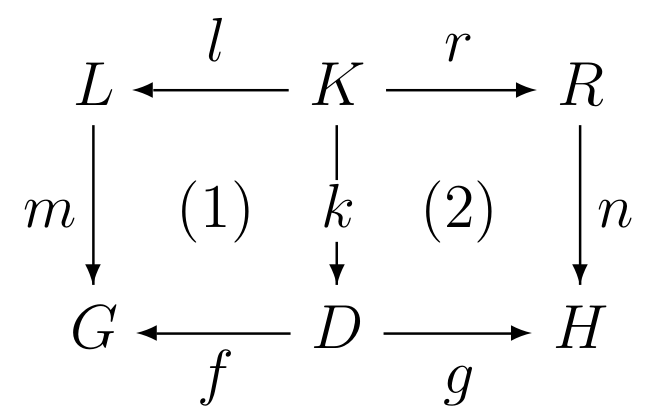
\includegraphics[width=0.44\textwidth]{figures/formal/dpo}
	\caption{Double pushout approach}
	\label{fig:dpo}
\end{figure}

We explain the components:
\begin{itemize}
\item L: The matcher of the rule
\item R: The rewriter of the rule
\item G: The graph to be matched/rewritten
\item H: The rewritten graph
\end{itemize}

Note that as it is not possible in DSLTrans rules to remove elements, $L = K$, and $G = D$.


\subsubsection*{Matcher of a Transformation Rule}

To create the actual matcher construct that will be matched during a rule's execution, the rule's \textit{Match} graph is combined with backward links, as well as any \textit{Apply} vertices connected to the backward links.

Note that the rule's NAC will also be considered in the matching of a rule.

\begin{definition}{Matcher of a Transformation Rule\\}
\label{def:matcher_transformation_rule}

Let the transformation rule $r = \big\langle \mathit{NAC}$, $\mathit{Match}$, $\mathit{Apply}$, $\mathit{backward}\big\rangle$.

Let $\mathit{Match}\star$ be the transitive closure of $\mathit{Match}$ to handle any indirect edges.

\bentley{Typed graph? Or copy the rule's structure? If it is a rule, note that it will not be well-formed. However, this is preferable to defining another structure to use}

We define $r$'s matcher, noted $\lceil r \rceil$, to be a typed graph six-tuple $\langle V,E,(s,t),\tau, \VT, \ET\rangle$, where:
\begin{itemize}
\item $V = V_{Match\star} \cup \big\{v \in V_{Apply} | \{\exists e \in E_{back} | s_{back}(e) = v\}\big\}$
\item $E = E_{Match\star} \cup E_{back}$
\item $s = s_{Match\star} \cup s_{back}$, $t = t_{Match\star} \cup t_{back}$
\item $\tau = \tau_{Match\star} \cup \tau_{Apply}$
\item $\VT = \VT_{Match\star} \cup \VT_{Apply}$
\item $\ET = \ET_{Match\star} \cup \ET_{Apply}$
\end{itemize}

\end{definition}

\subsubsection*{Rewriter of a Transformation Rule}

To continue with the double pushout approach, we must construct the rewriting (or replacement) graph.

The construction of this rewriter is essentially the same as the underlying rule. However, to support traceability, we require that backward links in the rule be converted into traceability links, and that new traceability links be created between all match and apply vertices. 

\begin{definition}{Rewriter of a Transformation Rule\\}
\label{def:rewriter_transformation_rule}

Let the transformation rule $r = \big\langle \mathit{NAC}$, $\mathit{Match}$, $\mathit{Apply}$, $\mathit{backward}\big\rangle$.

Let $\mathit{Match}\star$ be the transitive closure of $\mathit{Match}$ to handle any indirect edges.

We define $r$'s rewriter, noted $\lfloor r \rfloor$, to be a input-output model $\big\langle \mathit{Input}$, $\mathit{Output}$, $\mathit{trace}\big\rangle$, where:

\begin{itemize}
\item $ \mathit{Input} = \mathit{Match\star}$
\item $ \mathit{Output} = \mathit{Apply}$
\end{itemize}

We then modify $\mathit{trace}$ to contain the appropriate traceability links

\begin{itemize}
\item $E_{trace} = E_{backward} \cup \big\{e | \{$for each pair $m_i, a_j$ where $m_i \in V_{Match}, a_j \in V_{Apply}\}\big\}$
\item $s_{trace} = s_{backward} \cup \big\{a_j | \{$for each pair $m_i, a_j$ where $m_i \in V_{Match}, a_j \in V_{Apply}\}\big\}$
\item $t_{trace} = t_{backward} \cup \big\{m_i | \{$for each pair $m_i, a_j$ where $m_i \in V_{Match}, a_j \in V_{Apply}\}\big\}$
\end{itemize}

\bentley{Very messy}
\end{definition}

\subsubsection*{Application of a Transformation Rule (continued)}

\bentley{Fix up morphism notation. Is $\rightarrow$ good enough?} 
Recall that the interface graph K is equivalent to L due to the lack of deletion in DSLTrans rules. Thus, the l homomorphism is identity. The D correspondence graph will therefore be equivalent to G.


As well, we consider r to be a trivial homomorphism between the $\mathit{Match} \rightarrow \mathit{Input}$, $\mathit{Apply} \rightarrow \mathit{Output}$, and $\mathit{backward} \rightarrow \mathit{trace}$.

We also note here that a rule cannot be applied if there is a homomorphism between the rule's NAC and G. 

m is the typed graph homomorphism between the matcher of a rule $r$, denoted ($\lceil r \rceil$) and the $\mathit{Input}$ component of the input-output model

$n$ and $g$ will be homomorphism between their respective graphs. \bentley{This needs to be explained further. Maybe with a diagram?}

\subsubsection*{DSLTrans Layer Execution}

Now that the application of a particular DSLTrans rule has been explained, the next definition defines how a DSLTrans transformation layer executes. Recall that a layer is composed of rules, and acts on the current input-output model.


\begin{definition} {DSLTrans Layer Execution}
\label{def:dsltrans_layer_execution}


The execution of a DSLTrans layer can be defined as a function as follows:

\textit{applyLayer} : IOM $\times$ Layer $\rightarrow$ IOM

Let $l = \{r_0, r_1, \dots, r_n | r_i \in \textsc{Rules}\}$, $l \in \textsc{Layers}$.

Let $\mathit{IOM}_{Input}$, $\mathit{IOM}_{Output} \in \mathit{IOMs}$.

$\mathit{IOM}_{Output}$ will be the result of applying the production \textit{p} as defined below to $\mathit{IOM}_{Input}.$

We refer to the double-pushout literature for the creation of \textit{p}. Specifically, we refer to the definition of parallel direct derivations. This p will be created out of the productions created for each of the rules $r_i$ in the layer.

$p = \big\langle (p_1, {in}^1), \dots, (p_k, {in}^k) \big\rangle : (L \xleftarrow{l} L \xrightarrow{r} R)$

This collection of the rules is possible because DSLTrans rules do not delete anything. Essentially, a union is taken of the L, K, R components of each production.
\end{definition}

\begin{figure}[h!] \centering
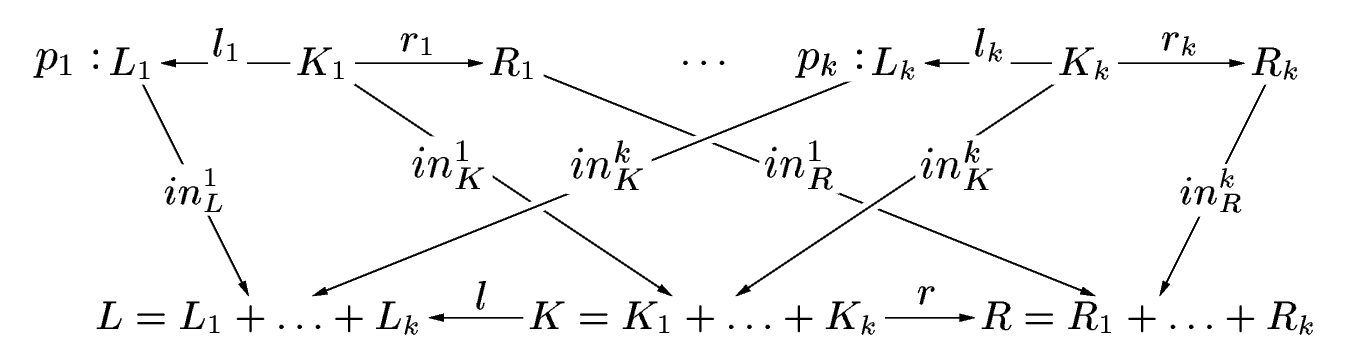
\includegraphics[width=0.44\textwidth]{figures/formal/parallel_productions}
	\caption{Parallel production \textit{p}}
	\label{fig:parallel_productions}
\end{figure}


\cref{def:dsltrans_layer_execution} is the core of DSLTrans' semantics, in which we build the result of executing a layer of a DSLTrans transformation. Many model transformation languages are based on graph rewriting, where the result of each rule rewrite is immediately usable by all other rules. In DSLTrans the result of executing one layer in DSLTrans is totally produced before the input to the layer is changed. This is enforced in \cref{def:dsltrans_layer_execution} by the fact that the layer production is composed of a union of the rule's productions. Rules belonging to the same layer are thus forced to execute independently, as described in the section on DSLTrans semantics.

\bentley{How does this handle different multiplicity of rule application?}


\subsubsection*{DSLTrans Transformation Execution}

Our final definition is for the execution of a DSLTrans transformation. Essentially, it is the chaining of layer executions applied on an input-output model.

We will begin by discussing the conditions for executing a model transformation on an input model.


\paragraph{Input Conditions}

For a well-formed transformation execution, we require the \textit{input-output model} in the domain to contain only an input graph. Recall that an \textit{input-output model} is the three-tuple $\big\langle \mathit{Input}$, $\mathit{Output}$, $\mathit{trace}\big\rangle$. We therefore require that both the $\mathit{Output}$ and $\mathit{trace}$ components in the domain IOM to be empty. This input-output model thus represents the first step of the transformation, where no rule has been executed yet.

The input-output model in the co-domain will contain this input graph, as well as the output graph and traceability links produced by the execution of the transformation. Let $\textsc{Execs}_t$ be the set of all well-formed input-output models produced for transformation $t$.

\begin{definition} {Execution of a DSLTrans Transformation\\}
\label{def:DSLTrans_transformation_execution} 

The execution of a model transformation is a function $\mathit{applyTransformation}: \mathit{IOM} \times \mathit{Transforms} \rightarrow \mathit{IOM}$.

This function is a chaining of executions of those layers within the transformation.

Recall the application of a layer is \textit{applyLayer} : IOM $\times$ Layer $\rightarrow$ IOM. Therefore, the application of a transformation is:

$\mathit{IOM}$ as input to chaining of layer executions \bentley{Is this function chaining? I don't know how to write the equation for this.}


\end{definition}


While the execution of the rules belonging to a layer happens in parallel, the execution of the layers of a transformation happens sequentially. As per \cref{def:DSLTrans_transformation_execution}, the input-output model that is the output of executing a given layer is passed onto the next layer as input. The final input-output model created will be the result of the model transformation.



\subsection{Confluence and Termination Properties}

We now prove two important properties about executions of transformations expressed in the subset of DSLTrans presented in this paper: \emph{confluence} and \emph{termination}. The proofs are provided at a high level, given the fact that DSLTrans essentially enforces both these properties by construction of the semantics of DSLTrans.

\begin{proposition}{Confluence}

Every model transformation execution is confluent up to typed graph isomorphism.

\bentley{As we are relying on the double-pushout approach, I think we get this confluence for free.}


\end{proposition}

\begin{pf}
We want to prove that for every model transformation execution of a transformation $\mathit{transform} \in \textsc{Transforms}$ having as input an input-output model $\mathit{input} \in \mathit{IOMs}$, its output is always the same up to typed graph isomorphism.\\


If we assume an execution of the transformation is not confluent then this should happen because of non-determinism when the execution of a transformation is being built. Non-determinism happens during the construction of a transformation execution at two points: 
\begin{enumerate}
\item The section `Execution of a DSLTrans Rule' discusses the matching and rewriting components to rule application. Note that our technique relies on the double-pushout approach, which itself is non-deterministic up to typed graph isomorphism, which does not contradict the proposition we are trying to prove. \bentley{Revise this.}


\item In Definition~\ref{def:dsltrans_layer_execution}, the rules composing a transformation layer are composed into a production on the input graph. Note that the order in which the transformation rules are composed may be non-deterministic. However, as these rules can be shown to be parallel independent \bentley{And they have to in that definition}, the production is by definition confluent up to typed graph isomorphism.

\end{enumerate}
Given there are no other sources of non-determinism when building the execution of a transformation, every model transformation execution is confluent up to typed graph isomorphism.
\end{pf}

\begin{proposition}{Termination}

Every model transformation execution terminates.
\end{proposition}
\begin{pf}
Let us assume that there is a transformation execution which does not terminate. In order for this to happen there must exist a part in the construction of the execution of a transformation which induces an algorithm with an infinite amount of steps. We identify three moments when this can happen:
\begin{enumerate}

\item If the matching and rewriting process of a rule is infinite. However, as the double-pushout approach uses a single production, then this must be a finite process. \bentley{Verify this, especially in the case of multiple applications of the rule.}

% if the result of the $match_{rl}(m_{in})$ function in definition~\ref{def:match_function} is an infinite set of match-apply graphs. The input-output model $m_{in}$ is by definition finite and the matching of each rule is independent from the execution of other rules in the same layer. As such, the number of subgraphs of $m_{in}$ isomorphic to $rl$'s matcher found during the execution of $rl$ is finite.


\item if Definition~\ref{def:dsltrans_layer_execution} of execution of a layer induces an infinite amount of steps. The only possibility for this to happen is if a layer has an infinite amount of transformation rules, which is a contradiction with Definition~\ref{def:layer}.

\item if Definition~\ref{def:DSLTrans_transformation_execution} of execution of a transformation induces an infinite amount of steps. Given layers are executed sequentially and no looping is allowed, the only possibility for this to happen is if the transformation has an infinite amount of layers, which contradicts Definition~\ref{def:transformation}.


\end{enumerate}
Given there are no other constructs in the semantics of a transformation that can induce an infinite amount of steps, every model transformation execution terminates.
\end{pf}

